\section{Erweiterungen}

\subsection{Qualität}

\subsubsection{Aufteilung in mehrere Django Apps}

Bereits in der Analyse (Abschnitt \ref{analyse:stand}) fiel auf, dass
das bestehende strongTNC Projekt aus einer einzigen Django App besteht. 
Innerhalb der App waren alle Models in einer
einzigen Datei enthalten (\texttt{models.py}), während die Views in mehrere
thematisch gruppierte Dateien aufgeteilt wurden (\texttt{device\_views.py},
\texttt{product\_views.py}, etc).\\
Diese Aufteilung der Views deutet darauf hin, dass die \texttt{tncapp} App für
mehrere thematisch unterschiedliche Bereiche zuständig ist, welche in der
Codebasis separiert werden könnten und sollten. Die Aufteilung in mehrere
Python-Dateien ist jedoch in Django Projekten der falsche Weg, um dies zu
erreichen. Stattdessen bietet Django für solche Fälle das Konzept einer App an.

Eine App ist ein Verzeichnis innerhalb eines Django Projektes, welches seine eigenen
Models, Views und Templates enthält. Die Apps werden in der
Projektweiten \texttt{settings.py} registriert. Ein einzelnes Projekt lässt sich
so in mehrere kleine MVC Container aufteilen.

Zusammenhängende Codeteile sollen wenn möglich in separate Apps unterteilt werden.
Dadurch werden die Apps \enquote{pluggable} und können aktiviert- und
deaktiviert werden kann. Die Separierung von Code in mehrere Apps
führt zu tiefer Kopplung\cite[S.~232--237]{larman2002applying}
und dadurch zu bessert wartbaren Code.

Aus den oben genannten Gründen haben wir die bestehende monolithische App in
folgende zehn moderat bis hoch kohäsiven Apps aufgeteilt:

\begin{itemize}
	\item \texttt{core}: Enthält Elemente, die von fast allen Apps
	verwendet werden, wie beispielsweise das \texttt{Session} Model oder die
	\texttt{WorkItemType} Klasse.
		
	\item \texttt{front}: Enthält alle Elemente zur Darstellung der Seiten, welche
	nicht App-spezifisch sind. Beispiele hierfür sind das Base-Template, der
	\texttt{highlight} Template Filter oder der \texttt{pagination} Ajax Endpoint.
	
	\item \texttt{auth}: Enthält Hilfsfunktionen, Mixins und Template Tags für die Authentisierung und Berechtigungsprüfung.
	
	\item \texttt{api}: Enthält Hilfsfunktionen und Mixins der API.
	
	\item \texttt{devices}: Enthält Models wie \texttt{Product}, \texttt{Device} und \texttt{Group} sowie dazugehörige Views.
		
	\item \texttt{filesystem}: Enthält Models und Code mit Bezug auf das
	Dateisystem (\texttt{File}, \texttt{Directory}, etc).
	
	\item \texttt{packages}: Enthält Models und Code zu Softwarepakete
	und deren verfügbaren Versionen.
		
	\item \texttt{policies}: Enthält Models und Code mit Bezug zu Policies und
	deren Durchsetzung mit Hilfe von Enforcements.
		
	\item \texttt{swid}: Enthält die Implementation der SWID Integration
	in strongTNC.
		
	\item \texttt{tpm}: Enthält Models für die TPM Integration in strongTNC. Diese
	App bietet aktuell noch keine Funktionalität.
\end{itemize}

\subsubsection{Verbesserung der Testing-Infrastruktur}
\label{improvements:tests}

Unit- und Integration-Tests sind zentral für die agile Entwicklung und für die
Sicherstellung der Wartbarkeit eines Softwareprojektes. Es wurde Zeit und
Aufwand in die Konfiguration der Testing-Umgebung investiert, um diese besser
und flexibler zu machen.

Die ursprüngliche Codebasis verwendete das
\texttt{unittest}\footnote{\url{https://docs.python.org/2/library/unittest.html}}
Modul aus der Python Standardbibliothek. Alle Tests befanden sich in einer
einzigen Datei.  Obgleich \texttt{unittest} eine stabile Lösung ist, fällt bei
der Verwendung auf, dass das stark von Java Unittests inspirierte Projekt,
relativ umständlich zu nutzen ist. Alle Tests müssen als Methoden in einer
Klasse geschrieben werden. Um Assertions zu definieren, müssen ebenfalls
Methodenaufrufe wie \texttt{assertEqual} oder \texttt{assertLessThan} verwendet
werden. Nachfolgend ein Minimalbeispiel:

\begin{listing}
\caption{Unittest Minimalbeispiel}
\label{improvements:unittest-beispiel}
\begin{pythoncode}
import unittest

class TestTheAnswer(unittest.TestCase):
    def testIt(self):
        self.assertEqual(19 + 23, 42)
\end{pythoncode}
\end{listing}

In Python gibt es jedoch bereits ein \texttt{assert} Keyword, welches beliebige
Assertions testen kann. Zudem ist es in Python üblich auf Klassen zu
verzichten, wenn sie keinen Mehrwert bieten. Im Fall von Tests ist es oft
sinnvoll , diese direkt als top-level Funktionen zu definieren und in mehrere
Module zu organisieren.

Um die Situation zu verbessern wurde die Test-Infrastruktur von
Unittest auf Pytest\footnote{\url{http://pytest.org/}} umgestellt. Das
Pytest Projekt beinhaltet Test-Discovery und -Ausführung, viele Hilfsfunktionen
und Unterstützung für Plugins.

Nachfolgend dasselbe Minimalbeispiel wie in Listing
\ref{improvements:unittest-beispiel}, mit Pytest:

\begin{listing}
\caption{Pytest Minimalbeispiel}
\label{improvements:pytest-beispiel}
\begin{pythoncode}
def test_the_answer():
    assert 19 + 23 == 42
\end{pythoncode}
\end{listing}

Falls mehrere Tests auf dieselben Daten zugreifen, kann wie bei Unittest eine
Klasse verwendet werden, es gibt jedoch noch eine weitere Möglichkeit: Fixtures.
Eine Fixture ist eine Funktion, deren Rückgabewert über \enquote{Dependency
Injection} einem Test übergeben wird. Eine selbst definierte Fixture könnte
beispielsweise folgendermassen aussehen:

\begin{listing}
\caption{Pytest Fixtures}
\label{improvements:pytest-fixtures}
\begin{pythoncode}
import pytest

@pytest.fixture
def database(self):
    conn = MyDatabaseConnection()
    return conn

def test_the_database(database):
    assert database.status() == 'OK'
\end{pythoncode}
\end{listing}

Ein weiteres, von uns häufig genutztes Feature, ist die Parametrisierung von
Tests. Ein \enquote{klassischer} Unittest könnte folgendermassen aussehen:

\begin{listing}
\caption{Kombinierte Tests}
\label{improvements:pytest-combined}
\begin{pythoncode}
import pytest

def test_add():
    assert 19 + 23 == 42
    assert 13 + 29 == 42
    assert 42 + 1 == 42
    assert 62 - 23 == 42
\end{pythoncode}
\end{listing}

Der Nachteil eines solchen Tests ist, dass obwohl vier verschiedene unabhängige
Bedingungen getestet werden, in einem Fehlerfall der gesamte Test als
\textit{failing} angezeigt wird.

Pytest bietet hier als Abhilfe parametrisierte Tests. Dabei werden, mit Hilfe eines
Decorators, aus einer einzelnen Funktion zur Laufzeit mehrere Tests generiert.

\begin{listing}
\caption{Parametrisierte Tests}
\label{improvements:pytest-parametrize}
\begin{pythoncode}
import pytest

@pytest.mark.parametrize(['a', 'b'], [
	(19, 23),
	(13, 29),
	(42, 1),
	(62, -23),
])
def test_add(a, b):
    assert a + b == 42
\end{pythoncode}
\end{listing}

In diesem Beispiel werden vier unabhängige Tests generiert. Drei davon sind
erfolgreich, während der Vierte einen Fehler meldet, da die Bedingung
\texttt{42 + 1 == 42} nicht erfüllt ist.

Um das Testen mit Django zu vereinfachen, wurde das \texttt{pytest-django}
Plugin verwendet. Es wurde ein \texttt{runtests.py} Script geschrieben, welches
die die Pfad-Variablen korrekt setzt, alle Tests ausführt und anschliessend die
Test Coverage anzeigt. \texttt{pytest-django} liefert Fixtures, wie \zb
\texttt{client} um auf einen Django Test Client zugreifen zu können oder
\texttt{transactional\_db}, um transaktionellen Zugriff auf die Datenbank zu
erhalten.

\subsubsection{Continuous Integration}

Eine Sicherstellung und langfristige Verbesserung der Softwarequalität ist nicht
möglich, wenn diese nicht regelmässig überprüft wird. Um dieses Ziel zu
erreichen, wurde in verschiedenen Bereichen auf \enquote{Continuous
Integration} (CI) gesetzt: Tests, Testabdeckung und statische Analyse.

\paragraph{Ausführung der Tests} \hspace{0pt} \\
\label{improvements:travis}
Um die Test Suite (Abschnitt \ref{improvements:tests}) automatisiert
auszuführen, wurde Travis CI\footnote{\url{https://travis-ci.org/}}
verwendet. Travis ist eine CI-Plattform mit Python-Unterstützung, die für Open
Source Projekte kostenfrei ist. Mit wenigen Zeilen in einer
Datei namens \texttt{.travis.yml} kann die Test-Ausführung konfiguriert werden.
Ein Fehlerfall wird auf Github angezeigt und der Autor des
entsprechenden Commits per E-Mail benachrichtigt.

\paragraph{Überwachen der Testabdeckung} \hspace{0pt} \\
Neben dem Testerfolg ist die Testabdeckung ebenfalls eine wichtige Kennzahl. Um
diese laufend zu überwachen wurde
Coveralls\footnote{\url{https://coveralls.io/}} verwendet. Coveralls bietet eine
Integration mit Travis CI und zeigt die Entwicklung der Testabdeckung an. Dank
einer Integration mit Github wird auch für jeden Pull Request die Veränderung
der Testabdeckung gemessen.

Die Testabdeckung für strongTNC ist inzwischen bei 70\% und stieg während der
gesamten Projektdauer kontinuierlich an:

\begin{figure}[H]
	\centering
	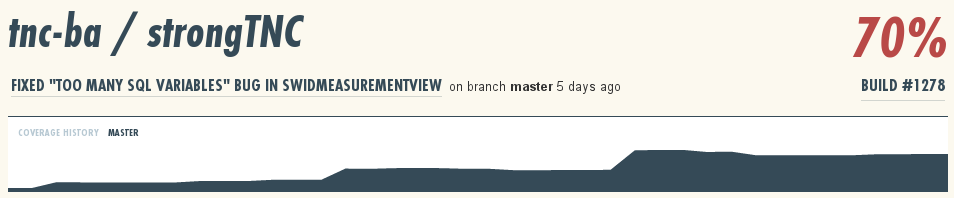
\includegraphics[width=\textwidth]{images/coveralls}
	\caption{Entwicklung der Testabdeckung}
	\label{improvements:coveralls}
\end{figure}

\paragraph{Messen der Codequalität} \hspace{0pt} \\
Neben Testing-Werkzeugen sind auch statische Codeanalyse-Tools hilfreich zur
Verbesserung der Codequalität. Sie erkennen häufige Schwachstellen im Code, wie
beispielsweise ungenutzte Variablen oder unerreichbaren Code.

Während der Entwicklung wurde bereits auf Tools wie
Pyflakes\footnote{\url{https://pypi.python.org/pypi/pyflakes}} und
Pylint\footnote{\url{http://www.pylint.org/}} gesetzt. Zusätzlich wurde das noch
junge Projekt Landscape\footnote{\url{https://landscape.io/}} eingebunden,
dieses überprüft den Code indem verschiedene Checks automatisch nach jedem Commit
ausgeführt werden. Den Report kann man über den Webbrowser betrachten und
analysieren.

\begin{figure}[H]
	\centering
	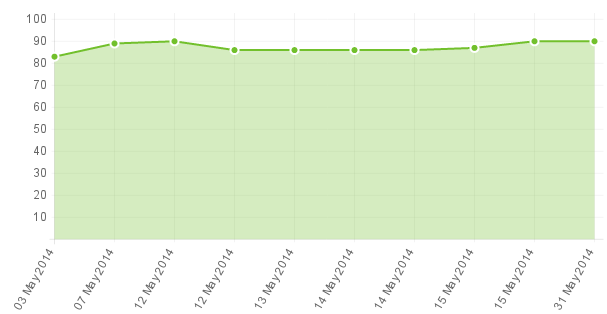
\includegraphics[width=0.6\textwidth]{images/landscape}
	\caption{Coveralls: Entwicklung des Landscape Quality Scores}
	\label{improvements:landscape}
\end{figure}

Auf Landscape liegt das Projekt aktuell bei einem Quality Score von 90\%.
Zu bemerken ist, dass Landscape einige False Positives liefert. Das
liegt daran, dass das Projekt noch jung ist und gewisse Spezialfälle -- welche in
einer dynamischen Sprache wie Python häufig vorkommen können -- nicht erkennt.
Zudem sind gewisse Kennzahlen, wie die maximale Zeilenlänge, noch nicht
konfigurierbar und werden deshalb als Fehler angezeigt, obwohl im Coding
Styleguide (Abschnitt \ref{anhang:coding-styleguide}) andere Regeln vereinbart
wurden. Damit sich diese Situation in Zukunft verbessert, wurden Feature
Requests für die entsprechenden Anpassungen
gestellt\footnote{\url{http://git.io/BqNWMw}, \url{http://git.io/O8MaNA}}.


\subsubsection{Deployment Dokumentation, Vagrant, Ansible}

Wenn man strongTNC in Produktion deployen will, müssen einige Dinge beachtet
werden. Beispielsweise sollte die Applikation nie ohne TLS produktiv über ein
Netzwerk genutzt werden, da die API Endpoints nur mit Hilfe von Basic Auth
geschützt sind.

Um den Nutzern von strongTNC in diesen Punkten eine Hilfestellung zu geben,
haben wir im Projekt-Repository ein Dokument mit allen nötigen Informationen
erstellt. Das Dokument findet sich im Repository unter
\texttt{doc/deployment.rst}\footnote{\url{https://github.com/strongswan/strongTNC/blob/master/docs/deployment.rst}}
sowie im Anhang dieser Dokumentation auf Seite
\pageref{anhang:deployment-manual}.

Falls man strongTNC jedoch nicht gleich produktiv nutzen will, sondern zuerst
testen möchte, wäre es etwas umständlich all diese Konfigurationsschritte
manuell durchzuführen. Für diesen Fall haben wir eine
Vagrant\footnote{\url{http://www.vagrantup.com/}}- und eine
Ansible\footnote{\url{http://www.ansible.com/}}-Konfiguration vorbereitet.
Vagrant ist ein Tool um die Erstellung und Konfiguration von Virtuellen
Maschinen zu automatisieren, während Ansible ein System zur Automation von
Deployments ist. Durch die Kombination der beiden Tools kann mit folgenden zwei
Befehlen eine komplett konfigurierte VM erstellt werden, mit welcher strongTNC
getetstet werden kann:

\begin{textcode}
$ cd /path/to/strongtnc/vagrant/
$ vagrant up
Bringing machine 'default' up with 'virtualbox' provider...
...
\end{textcode}

Alle weiteren Informationen befinden sich im Projekt-Repository unter
\texttt{vagrant/README.rst}\footnote{\url{https://github.com/strongswan/strongTNC/blob/master/vagrant/README.rst}}.

\subsubsection{Weitere Punkte}
\begin{description}

\item[Code Standards (PEP8)] Damit die Einhaltung der PEP8 Richtlinien
	garantiert ist, wurde eine entsprechende Prüfung in den Build Prozess
	integriert. Dadurch gilt ein Build als fehlgeschlagen, falls die Richtlinien
	nicht vollständig eingehalten wurden.

\item[Vermeidung von Hardcoded URLs] Gemäss Empfehlung des Django Frameworks
	soll das Verwenden von absoluten URLs in Templates und Views vermieden werden.
	Anstelle sollen URLs nur einmal, in der URLConf, konfiguriert und danach via
	Rückwärtssuche durch den Namen aufgelöst werden. Auf diese Weise können
	zentral Änderungen an URLs vorgenommen werden, ohne Templates oder Views
	anpassen zu müssen.

\item[Konsequente Frontend Validierung] Die bestehende Frontend Validierung
	wurde an diversen Orten inkonsequent oder fehlerhaft eingesetzt. Diese Mängel
	wurden behoben und damit die Validierung vereinheitlicht.

\item[Upgrade auf Django 1.6] strongTNC wurde von Django 1.5 auf Django 1.6
	aktualisiert. Die Codebasis ist so zukunftssicherer, kann neue Features nutzen
	und beinhaltet alle aktuellen Security-Fixes.

\end{description}

\subsection{Features}

\subsubsection{Aufteilung der Zugriffsrechte}
Um die Informationen in strongTNC zu Präsentationszwecken zugänglich zu machen,
ohne dass Änderungen vorgenommen werden können, weder absichtlich noch aus
Versehen, soll eine Readonly Rolle eingeführt werden.

In einem ersten Schritt soll ein Modell mit zwei Rollen eingeführt werden. Eine
Rolle für den readonly Zugriff und eine für den Vollzugriff. Die Rollen sollen,
so wie es gegenwärtig implementiert ist, nicht personalisiert sein. Die
Möglichkeit, den Login zu personalisieren sollte nicht grundsätzlich
ausgeschlossen werden, jedoch steht die Implementation eines nicht
personalisierten readonly Zugriffs im Vordergrund.

\paragraph{Technische Umsetzung} \hspace{0pt} \\
Das Django Webframework hat ein vollständiges Authentication- und
Permission-System integriert. Damit lassen sich komplexe Permission-Szenarien
abbilden, jedoch besteht auch die Möglichkeit, nur Teile daraus zu verwenden und
so ein einfacheres Rollen-Modell zu simulieren.

Da keine personalisierten Logins benötigt sind, werden zwei technische Benutzer
erstellt, die für die beiden Rollen eingesetzt werden. Die Namen der beiden Benutzer sind 
 \texttt{admin-user} und \texttt{readonly-user}. Dem
\texttt{admin-user} Benutzer wird eine \texttt{write\_access} Berechtigung erteilt, diese
kann in den Views mittels Django-Internem \texttt{@permission\_required()}
Decorator geprüft werden.

Diese Variante der Umsetzung erlaubt es, mit wenig Aufwand personaliserte Logins
einzuführen. Für die Verwaltung der Benutzer stellt Django ein Admin-Interface
zur Verfügung, die Benutzerverwaltung muss nicht selber entwickelt werden.

In den Templates können die Zugriffsrechte über das \texttt{perms} Objekt im
\texttt{Context} geprüft werden:

\begin{pythoncode}

    <p>Read-write access.</p>

\end{pythoncode}

Die zusätzliche Implementation eines Templatetags erleichtert die Steuerung von
HTML Formularelementen, deren Bedienung nur für schreibberechtigte Benutzer
erlaubt sein soll:

\begin{pythoncode}
@register.simple_tag(takes_context=True)
def input_editability(context):
    perms = context.get('perms', [])
    if 'auth.write_access' not in perms:
        return 'disabled="disabled"'
    return ''
\end{pythoncode}

Die Anwendung sieht wie folgt aus:

\begin{pythoncode}
<input type="text"name="name" value="{{ group }}"  />
\end{pythoncode}

Diese Umsetzung folgt einer Variation, des in \enquote{Security
Patterns}\cite{schumacher2013security} vorgeschlagenen Patterns \enquote{Full
Access With Errors}. Alle Funktionen sind stets für den Benutzer sichtbar.
Dadurch kann das User Interface einheitlich gestaltet werden und vermeidet auf
diese Weise mögliche Verwirrungen. Diejenigen Elemente, die der Benutzer nicht
bearbeiten darf, werden deaktiviert.

Um die beiden benötigten Benutzer initial zu erstellen, wurde das Django
Management-Kommando \texttt{setpassword} angepasst. Das Kommando erstellt direkt
die beiden Benutzer und erlaubt es, die Passwörter interaktiv oder per Parameter
festzulegen.

\paragraph{Alternativen} \hspace{0px} \\
Als Alternative zum Django Permission-System könnten auch die standardmässig
vorhandenen Flags \texttt{user.is\_admin} und \texttt{user.is\_staff} verwendet
werden. Dies wäre bedeutend einfacher zu implementieren, jedoch ist die Lösung
nicht ausbaufähig. Deshalb wird das Permission-System bevorzugt.

\subsubsection{Nachladen von grossen Datenmengen}
strongTNC muss mit grossen Datenmengen umgehen können. Wenn Datei-Messungen
durchgeführt- oder SWID Tags erfasst werden, ist beispielsweise die Zahl der
erfassten Dateien schnell im fünfstelligen Bereich. Wenn einzelne dieser Dateien
ausgewählt werden sollen, muss verhindert werden, dass immer die gesamte Menge
der Daten geladen wird.

\paragraph{Technische Umsetzung} \hspace{0pt} \\
Die gesuchten Datensätze werden mittels inkrementeller Suche per Ajax
nachgeladen.

Die Ajax Endpunkte wurden mit Hilfe der \enquote{Dajax-ice}\footnote{\url{http://www.dajaxproject.com/}} Django Erweiterung realisiert.
\enquote{Dajax-ice} stellt die nötigen Bibliotheken bereit, um Ajax Endpunkte wie gewöhnliche Views zu implementieren. So werden zum Beispiel benötigte HTTP Header
automatisch gesetzt und geprüft. Ausserdem generiert \enquote{Dajax-ice} Javascript Funktionen, welche die benötige Infrastruktur clientseitig bereitstellen, um Ajax Requests auszuführen.
\\

In Listing \ref{strongTNC:ajaxendpoint} ist die Beispielimplementation eines Ajax Endpoints zu sehen. Um auch bei Ajax Anfragen eine Authentifizierung zu erzwingen, wurde ein eigener Decorator (\texttt{@ajax\_login\_required}) erstellt. 
\begin{listing}
\caption{Beispiel eines Ajax Endpunktes}
\label{strongTNC:ajaxendpoint}
\begin{pythoncode}
@dajaxice_register
@ajax_login_required
def directories_autocomplete(request, search_term):
    dirs = Directory.objects.filter(path__icontains=search_term)
    results = {'results': [{'id': d.id, 'directory': d.path} for d in dirs]}
    return json.dumps(results)
\end{pythoncode}
\end{listing}

Clientseitig kann der Endpunkt wie folgt mit Javascript angesprochen werden:
\begin{listing}
\caption{Absenden eines Ajax Requests}
\begin{jscode}
Dajaxice.apps.filesystem.directories_autocomplete(callback, {search_term: 'system'});
\end{jscode} 
\end{listing}

Damit bei der inkrementellen Suche nicht bei jedem Tastenanschlag ein Request
abgesetzt wird, wurde ein Verzögerungsmechanismus implementiert, welcher erst einen Request
absetzt, wenn für eine bestimmte Zeit keine Eingabe mehr gemacht wurde (angelehnt an Nagle's Algorithmus \cite{nagle1984congestion}).
Durch die Minimierung der Anzahl HTTP Request, wird auch die Anzahl der teilweise komplexen und zeitintensiven Abfragen auf die Datenbank vermindert.

\paragraph{Langlaufende Operationen / Fehlerbehandlung}\hspace{0pt}\\
Asynchrone Aufrufe bringen zwei wesentliche Probleme mit sich. Zum einen kann es
sein, dass Fehler auftreten, wie z.B Timeouts, die der Benutzer nicht bemerkt.
Zum Anderen muss für den Benutzer ersichtlich sein, ob Datenübertragungen im
Hintergrund anstehen und falls ja, wann diese erfolgreich abgeschlossen sind.
Speziell für langlaufende Operationen durch datenbankintensive Abfragen oder
grosse Datenmengen, können Antwortzeiten im Sekundenbereich entstehen. \\
Zu diesem Zweck wurde eine Proxy Komponente \cite{gamma1994design}
implementiert, welche anstelle des eigentlichen Dajax-ice Aufrufes eingesetzt
wird. Komponenten, deren Inhalte per Ajax nachladen werden, werden vom Proxy mit
einem Statusindikator besetzt. Zusätzlich wurde ein globaler Statusindikator
eingeführt, der anzeigt, ob mindestens eine asynchrone Datenübertragung
stattfindet.\\
Treten Fehler bei einer Ajax Datenübertragung auf, wird der Benutzer mittels
Alert Box über den Fehler informiert.

\subsubsection{Ajax Pagination} 
Um grosse Datenmengen besser handhaben zu können, wurde die bestehende statische
Pagination durch eine dynamische, Ajax basierte Version ausgetauscht. Das Ziel
war, jegliche Art von Daten seitenweise auszuliefern, sowie die Datenmenge mit
Hilfe von Filtern dynamisch zu reduzieren. Bei der Architektur der
Pagingkomponente wurde darauf geachtet, dass diese wiederverwendet werden kann.
Der Inhalt, der seitenweise ausgeliefert werden soll, ist von der Pagination
entkoppelt und kann mittels einer Art Strategie (\enquote{Strategy Pattern}\cite{gamma1994design}) festgelegt werden.

\paragraph{Technische Umsetzung} \hspace{0pt} \\
Die Implementation der Paginination besteht aus den folgenden fünf Teilen:
\begin{enumerate}
	\item Javascript Frontend Komponente
	\item Template Tag, Templates und HTML Markup
	\item Generischer Ajax Endpunkt
	\item Individuelle Konfiguration pro Pagination Block
	\item \enquote{List Producer} für die Datenaufbereitung, wiederverwendbar
\end{enumerate}

\autoref{paginationSequence} zeigt den Grobablauf beim dynamischen Anfordern einer
neuen Seite.

\begin{figure}[H]	
	\centering
	\begin{tikzpicture}
	\begin{umlseqdiag}

		% Objekte

		\umlobject[x=0]{Javascript}
		\umlobject[x=4]{HTMLPage}
		\umlobject[x=7]{AjaxEndpoint}
		\umlobject[x=11]{ConfigRegistry}
		\umlobject[x=13]{Config}
		\umlobject[x=15]{Producer}
		
		% Calls
		\begin{umlfragment}[type=loop, label=foreach container, inner ysep=6]
		\begin{umlcall}[dt=16, padding=4, op=readPagingConfig(), return=confName]{Javascript}{HTMLPage}
		\end{umlcall}
		\end{umlfragment}
		
		\begin{umlcall}[dt=14, type=asynchron, op={getPage(confName, pageNo)}]{Javascript}{AjaxEndpoint}
		
			\begin{umlcall}[padding=3, op=getConf(confName),return=conf]{AjaxEndpoint}{ConfigRegistry}
			\end{umlcall}
				
			\begin{umlcall}[dt=5, padding=3, op=getProducer(), return=Producer]{AjaxEndpoint}{Config}
			\end{umlcall}	
				
			\begin{umlcall}[dt=5, padding=3, op={getDataSlice(from, to)}, return=dataSlice]{AjaxEndpoint}{Producer}
			\end{umlcall}
			
			\begin{umlcall}[dt=5, padding=3, op=getTemplate(), return=template]{AjaxEndpoint}{Config}
			\end{umlcall}
			
			\begin{umlcallself}[dt=5, padding=3, op={renderToHtml(template, dataSlice)}]{AjaxEndpoint}
			\end{umlcallself}
			
			\begin{umlcall}[padding=3, type=return, op=HTML]{AjaxEndpoint}{Javascript}
			\end{umlcall}
			
		\end{umlcall}
		
		\begin{umlcall}[dt=5, padding=3, op={setNewHTML(HTML)}]{Javascript}{HTMLPage}
		\end{umlcall}
			
	\end{umlseqdiag}
\end{tikzpicture}

	\caption{Sequenzdiagramm, Grobablauf}
	\label{paginationSequence}
\end{figure}


\begin{description}
	\item[HTMLPage] Auf der HTML Seite werden Container definiert, welche später
	mit den Seiteninhalten befüllt werden. Die Container können entweder direkt in
	HTML (Listing~\ref{paging:container}) definiert werden oder mittels, des dafür
	kreierten, Template Tags (Listing~\ref{paging:templatetag}) generiert werden,
	üblicherweise sollte der Template Tag verwendet werden.
\begin{listing}[H]
\caption{Pagination HTML Markup}
\label{paging:container}
\begin{htmlcode}
<div class="ajax-paged"
  data-config="regid_list_config"
  data-args="{}"
  data-initial="True"
  data-urlparams="True"
  data-filter="True">
	[...]
	<div class="paged-content"></div>
	[...]
</div>
\end{htmlcode}
\end{listing}

\begin{listing}
\caption{Verwendung eines \enquote{Paged Blocks} mittels Template Tag}
\label{paging:templatetag}
\begin{pythoncode}

\end{pythoncode}
\end{listing}

	\item[Javascript] Eine Aufgabe der Javascript Komponente ist das Auslesen aller
	Paged Block Konfigurationen aus dem DOM der aktuellen HTML Seite. Identifiziert
	werden diese Blöcke durch die CSS Klasse \texttt{ajax-paged}. Es können mehrere
	Paged Block Komponenten pro Seite definiert werden. Für jeden der gefunden
	Paging Container wird ein Javascipt Pager-Objekt instanziert, welches für die
	Verwaltung des Zustandes -- zum Beispiel die aktuelle Seite -- und die
	Kommunikation mit dem AjaxEndpoint verantwortlich ist. Nach erfolgreicher
	Kommunikation mit dem AjaxEndpoint wird der zurückgelieferte HTML Block in den
	entsprechenden Container geladen. 

	\item [AjaxEndpoint] Der AjaxEndpoint nimmt Requests entgegen und kann anhand
	des übergebenen Konfigurationsnamens die zugehörige Konfiguration laden. Diese
	beinhaltet einen Producer und die Referenz auf ein Template. Die
	Datengenerierung wird an den Producer delegiert, dieser übernimmt auch die
	Unterteilung der Daten in die Angeforderte  Seiten grösse. Die Daten, welche der
	Producer zurück gibt werden anschliessend als Kontext verwendet, um das
	Template in HTML zu rendern. Durch diese Separierung wird eine hohe
	Wiederverwendbarkeit erreicht. Verschiedene Datenquellen und Templates können
	kombiniert und wiederverwendet werden.
\begin{listing}
\caption{Beispiel einer Paging Config}
\begin{pythoncode}
regid_list_paging = {
    'template_name': 'front/paging/default_list',
    'list_producer': regid_producer_factory.list(),
    'stat_producer': regid_producer_factory.stat(),
    'url_name': 'swid:regid_detail',
    'page_size': 50,
}
\end{pythoncode}
\end{listing}

	\item[Producer] Die Datenaufbereitung, Datenbankabfragen, Slicing der Daten in
	Seiten und vorgängiges Filtern sind im Producer definiert. Durch ein
	gemeinsames Producer Interface (impliziter Contract\cite{contracts:2003}),
	können Producer flexibel ausgetauscht und wiederverwendet werden. Eine konkrete
	Implementation eines Producers ist in Listing~\ref{paging:producer} zu sehen.
	
\begin{listing}
\caption{Beispielimplementation eines Producers}
\label{paging:producer}
\begin{pythoncode}
def swid_files_list_producer(from_idx, to_idx, filter_query, dynamic_params, static_params=None):
 if not dynamic_params:
     return []
 tag_id = dynamic_params['tag_id']
 return Tag.objects.get(pk=tag_id).files.all()[from_idx:to_idx]
\end{pythoncode}
\end{listing}
	
	Für generische List Producer, welche lediglich eine Liste von Objekten eines
	bestimmten Models liefern, wurde eine eine \enquote{Factory} erstellt:
	
\begin{listing}
\caption{Producer Factory}
\begin{pythoncode}
swid_producer_factory = ProducerFactory(Tag, 'unique_id__icontains')
swid_producer_factory.list()
\end{pythoncode}
\end{listing}
	

\end{description}

%\paragraph{Ablauf} \hspace{0pt} \\
%Um einen Pagination Block in eine Seite einzubinden, existiert ein Template Tag.
%Dieser inkludiert einen vorgegeben HTML Block und überträgt allfällige
%Konfigurationen in Daten-Attribute des HTML Blocks.\\
%Ein so eingebundener Block wird durch die Javascript Komponente gefunden und die
%Pagination wird initialisiert.
%
%Konfiguriert wird eine Pagination Instanz über ein \enquote{Config-Dictionary}.
%Dieses muss an zwei Stellen referenziert werden. Einerseits wird dieses im
%Template Tag angegeben, andererseits muss die Konfiguration im Ajax Endpunkt
%registriert werden.
%
%Die Javascript Komponente übermittelt den Namen der Konfiguration, den Index der
%angeforderten Seite, sowie optionale kontextabhängige Variablen zum Ajax
%Endpunkt.

\subsubsection{Models für MySQL Support}
\paragraph{Empfehlung für Wechsel der Datenbank} \hspace{0pt} \\
Die enge Kopplung von strongSwan und strongTNC durch eine gemeinsam genutzte
Datenbank, hat zur Folge, dass Anpassungen des Datenbankschemas, Änderungen an
allen Komponenten bedingen. Des Weiteren ist zu erwarten, dass für grössere
Installationen SQLite zu leichtgewichtig ist. Optimierungen und Profiling sind
eingeschränkt durchführbar, zu dem wird keine referenzielle Integrität
unterstützt. Problematisch ist auch, dass SQLite nicht mehrbenutzerfähig ist.

\paragraph{Generierung des Datenbankschemas} \hspace{0pt} \\
Django unterstützt diverse Datenbankbackends
\footnote{\url{https://docs.djangoproject.com/en/1.6/ref/databases/}}, unter
anderem MySQL, PostgreSQL, MSSQL und das zur Zeit verwendete SQLite. Wir
empfehlen das SQLite Backend möglichst bald durch ein anders Datenbankbackend zu
ersetzen. Aus diesem Grund wurden die Django Models so angepasst, dass sie dem
aktuellen Datenbankschema entsprechen. Das Django ORM kann daraus
datenbankspezifisches SQL-DDL generieren, und so die Migration erheblich
erleichtern.

\subsubsection{Split der Configfiles}

Um beim Deployment von strongTNC den Code und die Konfiguration trennen zu
können, sollte man die Möglichkeit haben, wichtige Einstellungen wie die
Datenbank-Connection-Strings, in einer nicht versionierten Datei zu
konfigurieren. Drei verbreitete Möglichkeiten sind:

\begin{itemize}
	\item Konfiguration über Umgebungsvariablen, wie es durch die \enquote{12
		Factor App} Methodologie empfohlen
		wird\footnote{\url{http://12factor.net/config}}.
	\item Eine \texttt{settings\_local.py} Datei, welche alle Konfigurationen von
		der regulären \texttt{settings.py} Datei importiert und zu konfigurierende
		Werte überschreibt.
	\item Eine \texttt{settings.ini} Datei, welche durch die \texttt{ConfigParser}
		Klasse aus der Python Standardbibliothek geparsed wird.
\end{itemize}

Die erste Methode ist äusserst gut geeignet wenn man seine Applikation auf einem
Cloud-Hosting Provider wie Heroku deployen will. Für Systemadminstratoren, die
sich Konfigurationsdateien gewöhnt sind, ist dies allerdings etwas umständlich.

Die zweite Möglichkeit bietet grosse Flexibilität, weist jedoch auch Gefahren
auf, da in einer solchen Datei beliebiger Code ausgeführt werden kann.

Wir haben deshalb den dritten Ansatz gewählt: Eine \texttt{settings.ini} Datei,
welche lediglich nichtausführbare Konfigurationsdaten enthält. Die Datei darf
sich entweder im Projektverzeichnis oder im \texttt{/etc/strongTNC/} Verzeichnis
befinden. Eine Beispielkonfiguration mit dem Namen \texttt{settings.sample.ini}
wird mit strongTNC mitgeliefert.

\subsubsection{Weitere Punkte}
\begin{description}
\item[Django Admin-Interface] Django bietet die Möglichkeit, die Datenbank über
ein automatisch generiertes Admin-Interface zu verwalten. Auf diese Weise
können potentiell fehleranfällige Datenmanipulationen per SQL vermieden
werden. Die Models wurden mit den nötigen Metadaten erweitert, damit dieses
Feature aktiviert werden konnte.

\item[Erstellen von Files und Versions] Bisher war es nicht möglich über die
Oberfläche von strongTNC neue Files und neue Versionen zu erstellen. Die
Ansichten wurden um diese Funktionalität ergänzt.

\item[Verknüpfung von Daten in Views] Die Views wurden durch sinnvolle
Verknüpfungen ergänzt. Die  Verknüpfungen waren bereits in der Datenbank
vorhanden, jedoch in den Views nicht direkt ersichtlich, so zum Beispiel welche
Enforcements einer Gruppe zugeordnet sind.

\item[URL Hash Parameter] Um Parameter in der URL abzulegen und auszulesen,
wurde eine Javascript Hilfsbibliothek erstellt. Die Bibliothek erlaubt es, die
Parameter in der URL abzulegen ohne einen Reload auszulösen. Ausserdem kann auf
Änderungen eventbasiert (Observer Pattern \cite{gamma1994design}) reagiert werden.
Änderungen welche mittels Ajax ausgelöst und somit keinen Reload zur Folge
haben, können so über die URL und die Browser History zugänglich gemacht werden.

\item[Umstellung auf UTC] Die bestehende Konfiguration von strongTNC hatte keine
Unterstützung für Zeitzonen. Dies stellt ein Problem dar, wenn sich Clients aus
verschiedenen Zeitzonen in das Netzwerk einwählen. Mit unseren Anpassungen
bietet strongTNC vollständige Unterstützung für Zeitzonen und stellt alle Zeiten
gemäss der konfigurierten Zeitzone dar.

\end{description}




